\documentclass[12pt,a4paper]{article}

% ─── 1. PACKAGES ──────────────────────────────────────────────────────────────
\usepackage[utf8]{inputenc}
\usepackage[T1]{fontenc}
\usepackage{amsmath, amssymb}
\usepackage{geometry}
\usepackage{graphicx}
\usepackage{xcolor}
\usepackage{listings}
\usepackage{hyperref}
\usepackage{booktabs}
\usepackage{enumitem}
\usepackage{tcolorbox}
\usepackage{mdframed}
\usepackage{fancyhdr}
\usepackage{titlesec}
\usepackage{tikz} 
\usetikzlibrary{shapes.geometric, positioning, arrows.meta, calc, decorations.pathreplacing}

% Font Settings
\usepackage{newtxtext,newtxmath} % Times New Roman
\usepackage{courier}             % Courier New untuk kode

\geometry{margin=2.5cm}

% ─── 2. WARNA TEMA ────────────────────────────────────────────────────────────
\definecolor{codebg}{RGB}{245,247,250}
\definecolor{codeframe}{RGB}{180,195,215}
\definecolor{keywordcolor}{RGB}{0,112,192}
\definecolor{commentcolor}{RGB}{100,160,100}
\definecolor{stringcolor}{RGB}{180,70,50}
\definecolor{notebg}{RGB}{255,249,230}
\definecolor{noteframe}{RGB}{230,180,50}
\definecolor{tipbg}{RGB}{230,245,235}
\definecolor{tipframe}{RGB}{50,160,90}
\definecolor{sectioncolor}{RGB}{30,80,150}

% ─── 3. STYLE SECTION & TOC ───────────────────────────────────────────────────
\titleformat{\section}{\Large\bfseries\color{sectioncolor}}{}{0em}{\thesection\quad}[\titlerule]
\titleformat{\subsection}{\large\bfseries\color{sectioncolor!80}}{}{0em}{\thesubsection\quad}

% Style Table of Contents
\usepackage{tocloft}
\renewcommand{\cftsecleader}{\cftdotfill{\cftdotsep}}
\renewcommand{\cftsecfont}{\bfseries\color{sectioncolor}}

% ─── 4. LISTINGS (CODE STYLE) ─────────────────────────────────────────────────
\lstdefinestyle{customstyle}{
  basicstyle=\ttfamily\small,
  backgroundcolor=\color{codebg},
  frame=single,
  rulecolor=\color{codeframe},
  keywordstyle=\bfseries\color{keywordcolor},
  commentstyle=\itshape\color{commentcolor},
  stringstyle=\color{stringcolor},
  numbers=left,
  numberstyle=\tiny\color{gray},
  breaklines=true,
  tabsize=4,
  showstringspaces=false
}
\lstset{style=customstyle}

% ─── 5. KOTAK CATATAN (MD-FRAME) ──────────────────────────────────────────────
\newmdenv[
  backgroundcolor=notebg, linecolor=noteframe, linewidth=2pt,
  leftline=true, topline=false, rightline=false, bottomline=false,
  innerleftmargin=10pt, innertopmargin=6pt, innerbottommargin=6pt, skipabove=8pt
]{notebox}

\newmdenv[
  backgroundcolor=tipbg, linecolor=tipframe, linewidth=2pt,
  leftline=true, topline=false, rightline=false, bottomline=false,
  innerleftmargin=10pt, innertopmargin=6pt, innerbottommargin=6pt, skipabove=8pt
]{tipbox}

% ─── 6. HEADER & FOOTER ───────────────────────────────────────────────────────
\pagestyle{fancy}
\fancyhf{}
\fancyhead[L]{\small\textit{Pengantar Data Science}}
\fancyhead[R]{\small\textit{noteify -- Kausalitas \& Studi Observasional}}
\fancyfoot[C]{\thepage}
\renewcommand{\headrulewidth}{0.4pt}

% ─── 7. DATA COVER ────────────────────────────────────────────────────────────
\title{
  {\LARGE\bfseries PENGANTAR DATA SCIENCE}\\[0.5em]
  {\large Modul Pembelajaran: Asosiasi, Kausalitas, dan Desain Studi}\\[0.8em]
  {\normalsize Penjelasan komprehensif mengenai konsep dasar sains data, perbedaan asosiasi dan kausalitas, eksperimen terkontrol, serta bahaya dari korelasi palsu (\textit{spurious correlations}).}
}
\author{}
\date{}

% ==============================================================================
\begin{document}

\maketitle
\thispagestyle{fancy}
\tableofcontents
\newpage

% ─── KONTEN MATERI ─────────────────────────────────────────────────────────────

\section{Apa itu Data Science?}


Pada tingkat yang paling mendasar, \textbf{Data Science} (Ilmu Data) adalah proses penarikan kesimpulan dari informasi yang tidak sempurna (\textit{imperfect information}). 

Sejak awal peradaban, manusia selalu berusaha memperkirakan dan menebak hasil dari suatu kejadian berdasarkan informasi yang cacat atau tidak lengkap. Lalu, apa yang membuat Data Science modern menjadi bidang yang berbeda, baru, dan sangat esensial saat ini? Jawabannya terletak pada \textbf{penemuan perangkat komputasi yang sangat kuat} dan \textbf{teknik statistik yang tangguh (robust)}. Alat-alat inilah yang memungkinkan kita untuk menarik kesimpulan tersebut secara sistematis, terukur, dan dapat diandalkan (\textit{reliably}).

\newpage
\section{Terminologi Inti dalam Studi Observasional}

Sebelum Anda menganalisis data apa pun, Anda harus mendefinisikan komponen-komponen penyusun studi Anda. Terdapat tiga istilah sangat krusial yang akan terus digunakan dalam dunia analisis data dan eksperimen:

\begin{table}[h]
\centering
\begin{tabular}{@{}p{3.5cm}p{11cm}@{}}
\toprule
\textbf{Istilah} & \textbf{Definisi \& Penjelasan} \\ \midrule
\textbf{Individuals} \newline \textit{(Individu/Unit)} & Subjek spesifik yang sedang Anda teliti. Sering juga disebut sebagai partisipan atau unit. Walaupun sering kali berupa manusia, individu bisa berupa apa saja, seperti mobil, benda, sel, atau bahkan perusahaan. \\ \addlinespace
\textbf{Treatment} \newline \textit{(Perlakuan)} & Faktor, variabel, atau intervensi yang Anda curigai sebagai \textbf{penyebab} dari hasil tertentu. Contohnya: konsumsi cokelat, pemberian vaksin COVID-19, atau keanggotaan dalam organisasi internasional seperti NATO. \\ \addlinespace
\textbf{Outcome} \newline \textit{(Hasil/Dampak)} & Efek akhir atau hasil yang sedang Anda ukur dari subjek. Contohnya: apakah seseorang terkena penyakit jantung atau tidak, sembuh atau tidak, dsb. \\ \bottomrule
\end{tabular}
\caption{Terminologi Dasar dalam Studi Data}
\end{table}

\newpage
\section{Asosiasi vs. Kausalitas (Studi Kasus Cokelat)}


[Image of Correlation vs Causation diagram]


Salah satu tantangan terbesar dan paling sering disalahpahami dalam ranah \textit{Data Science} adalah \textbf{membuktikan secara definitif bahwa sebuah perlakuan (treatment) benar-benar menyebabkan sebuah hasil (outcome)}.

\subsection{Studi dan Meta-Analisis Cokelat}
Pada bulan Juli 2020, sebuah artikel di \textit{European Journal of Preventive Cardiology} melakukan sebuah "meta-analisis". Artinya, mereka mengagregasi (menggabungkan) data dari beberapa studi independen sebelumnya untuk bekerja dengan himpunan data (\textit{dataset}) yang sangat besar.
\begin{itemize}
    \item \textbf{Subjek (Individuals):} 336.289 orang dewasa dari AS, Swedia, dan Australia.
    \item \textbf{Temuan Utama:} Peneliti mengobservasi bahwa orang-orang yang rutin memakan cokelat memiliki \textbf{risiko serangan jantung 8\% lebih rendah}.
\end{itemize}

\subsection{Mendefinisikan Asosiasi (Sebuah "Hubungan")}
Tajuk berita awal (headline) dari studi tersebut menyatakan bahwa makan cokelat \textbf{"dikaitkan" (linked)} dengan risiko serangan jantung yang lebih rendah. 
\textbf{Asosiasi (atau relasi/hubungan):} Ini semata-mata berarti bahwa dua hal bergerak bersamaan atau memiliki hubungan matematis. Data secara tulen menunjukkan bahwa kelompok individu yang makan cokelat juga mengalami lebih sedikit penyakit jantung. \textbf{Namun, ini tidak membuat klaim apapun tentang MENGAPA mereka bergerak bersama.}

\subsection{Lompatan Menuju Kausalitas (Sebab-Akibat)}
Masalah besar muncul ketika berbagai media berita (seperti \textit{European Society of Cardiology} dan \textit{National Safety Council}) menulis ulang tajuk berita tersebut menjadi \textit{"Cokelat baik untuk jantung"} dan \textit{"Apakah makan cokelat menyehatkan jantung? Studi mengatakan 'ya'"}.

\textbf{Kausalitas (Causation):} Tajuk berita baru ini membuat klaim yang jauh lebih kuat dan berbahaya. Mereka menyiratkan bahwa tindakan memakan cokelat secara aktif mengarah pada atau \textbf{menyebabkan} penurunan penyakit jantung. Ini memberi kesan (\textit{suggesting}) bahwa meningkatkan asumsi cokelat Anda akan secara langsung memperbaiki kesehatan Anda.

\subsection{Kecacatan Berita: Kausalitas Terbalik (Reverse Causation)}
Dr. Alice Lichtenstein, seorang profesor ilmu gizi, menunjukkan kecacatan fatal dalam mengasumsikan kausalitas dari data observasional ini. Beliau menyoroti kemungkinan terjadinya \textbf{Kausalitas Terbalik (\textit{Reverse Causation})}.

Jika seseorang sudah memiliki penyakit jantung, dokter mereka kemungkinan besar akan menasihati mereka untuk berhenti makan makanan manis seperti cokelat. Oleh karena itu, \textbf{memiliki penyakit jantung mungkin MENYEBABKAN seseorang makan lebih sedikit cokelat}, bukan sebaliknya (makan cokelat mencegah penyakit jantung). 

\begin{notebox}
\textbf{Poin Kunci:}\\
Tanpa mengendalikan variabel-variabel kondisi pasien ini, Anda tidak bisa tahu ke arah mana arus kausalitas itu mengalir. Korelasi (Asosiasi) BUKANLAH Kausalitas!
\end{notebox}

\newpage
\section{Membuktikan Kausalitas: Penemuan Kolera John Snow}


Untuk memahami bagaimana cara *benar-benar* membuktikan kausalitas, kita akan mengeksplorasi salah satu contoh \textit{data science} paling awal dan paling terkenal di dunia: Epidemi Kolera di London pada tahun 1850-an.

\subsection{Teori Miasma dan Obat-Obatan Liar}
Pada era 1850-an, keberadaan bakteri dan kuman belum diketahui oleh sains. Hipotesis yang mendominasi saat itu adalah \textbf{Teori Miasma}, yang menyalahkan penyebaran penyakit pada bau busuk yang dipancarkan oleh limbah dan materi busuk di udara.
\begin{itemize}
    \item \textbf{Penganut Terkenal:} Florence Nightingale (yang kemudian membersihkan rumah sakit agar tidak bau) dan Edwin Chadwick (Komisaris Dewan Kesehatan, yang membersihkan sistem pembuangan kotoran).
    \item \textbf{Obat-obatan Historis yang Mengada-ada:} Karena percaya "bau" adalah pelakunya, orang-orang mengusulkan solusi liar: melarikan diri ke tempat berudara bersih, membawa saku penuh bunga ("posies"), mengambil udara bersih dalam tong dari Menara Eiffel, atau menembakkan tong mesiu ke langit untuk mengganti bau busuk.
\end{itemize}

\begin{tipbox}
\textbf{Paralel Modern (COVID-19):}\\
Perilaku manusia tetap bisa diprediksi. Di masa-masa awal COVID-19, pengobatan yang belum terbukti juga menyebar dengan cepat karena panik: menyuntikkan disinfektan, menjemur tubuh di bawah sinar matahari ekstrem, \textit{hydroxychloroquine}, makan/menghindari es krim, hingga bernapas dalam-dalam sebelum batuk (seperti yang disarankan J.K. Rowling).
\end{tipbox}

\subsection{Peta Broad Street}
Seorang dokter bernama \textbf{John Snow} meragukan teori miasma. Ia memperhatikan bahwa rumah-rumah yang bersebelahan persis bisa memiliki tingkat kematian yang sangat berbeda—hal yang sama sekali tidak masuk akal jika penyebabnya adalah "bau busuk" yang melayang bebas di udara. Selain itu, gejala kolera (diare dan muntah) mengindikasikan penyakit ini "ditelan" masuk ke pencernaan, bukan dihirup.

\textbf{Visualisasi Data:} Snow menciptakan salah satu visualisasi data pertama dalam bidang epidemiologi. Ia memetakan kematian kolera sebagai batang hitam kecil pada peta jalan \textit{Broad Street}, London.

\textbf{Anomali:} Ia mencatat bahwa kematian berkerumun sangat padat di sekitar pompa air \textit{Broad Street}. Menariknya, sebuah tempat pembuatan bir (\textit{brewery}) di dekatnya memiliki NOL kematian. Mengapa? Karena para pekerja di sana minum bir yang mereka buat sendiri atau memiliki sumur pribadi yang tidak terkontaminasi.

\textbf{Intervensi Pertama:} Snow meminta agar gagang pompa air \textit{Broad Street} dicabut sehingga orang tidak bisa menggunakannya. Kasus kolera langsung turun drastis. Namun, karena epidemi tersebut memang secara alami sedang mereda, kaum skeptis berargumen bahwa hal ini belum secara ketat membuktikan kausalitas.

\subsection{"Eksperimen Agung" Snow (The Gold Standard)}
Untuk menetapkan kausalitas yang tak terbantahkan, Snow "zoom out" untuk mempelajari seluruh kota London dan melihat dua perusahaan penyedia air yang saling tumpang tindih (\textit{overlapping}): \textbf{Southwark \& Vauxhall (S\&V)} dan \textbf{Lambeth}.

\textbf{Mengendalikan Variabel (Controlling for Variables):} Karena pipa air dari kedua perusahaan ini melayani lingkungan yang saling tumpang tindih dan identik, Snow dapat mengendalikan variabel demografi, genetika, dan pendapatan.

\begin{figure}[h]
    \centering
    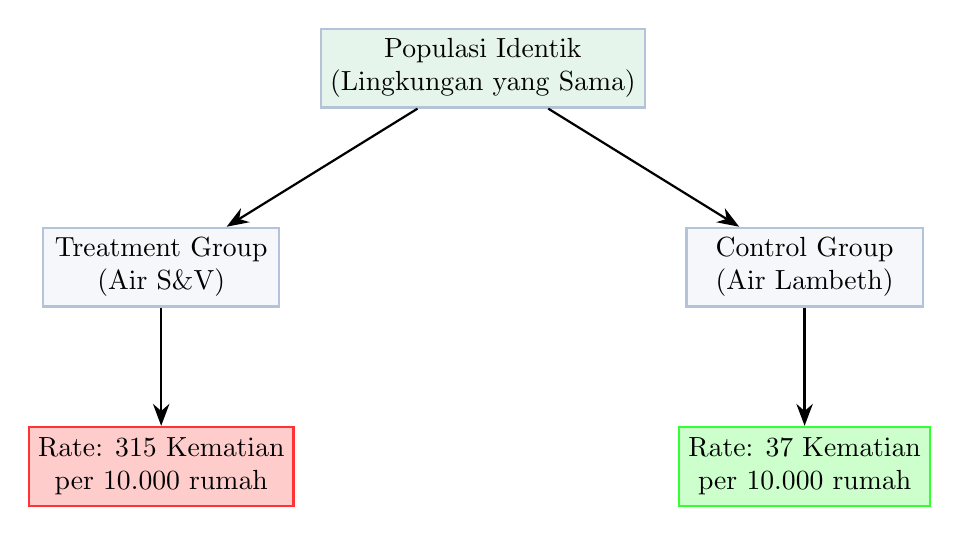
\begin{tikzpicture}[
        box/.style={draw, rectangle, minimum width=3cm, minimum height=1cm, align=center, fill=codebg, draw=codeframe, thick},
        arr/.style={-{Stealth[scale=1.2]}, thick}
    ]
    
    % Population
    \node[box, fill=tipbg] (pop) {Populasi Identik\\(Lingkungan yang Sama)};
    
    % Groups
    \node[box] (sv) [below left=1.5cm and 0.5cm of pop] {Treatment Group\\(Air S\&V)};
    \node[box] (lam) [below right=1.5cm and 0.5cm of pop] {Control Group\\(Air Lambeth)};
    
    % Outcomes
    \node[box, fill=red!20, draw=red!80] (out1) [below=1.5cm of sv] {Rate: 315 Kematian\\per 10.000 rumah};
    \node[box, fill=green!20, draw=green!80] (out2) [below=1.5cm of lam] {Rate: 37 Kematian\\per 10.000 rumah};

    % Arrows
    \draw[arr] (pop) -- (sv);
    \draw[arr] (pop) -- (lam);
    \draw[arr] (sv) -- (out1);
    \draw[arr] (lam) -- (out2);

    \end{tikzpicture}
    \caption{Desain Observasi Terkontrol pada Eksperimen Agung John Snow.}
\end{figure}

\textbf{Menggunakan Tingkat (Rate) vs Angka Mentah (Raw Counts):} 
S\&V memiliki 1.263 kematian, sementara Lambeth 98. Namun, karena perusahaan melayani jumlah rumah yang berbeda, angka mentah akan sangat menyesatkan. Snow menghitung \textit{Rate} (Tingkat: kematian per 10.000 rumah). Hasilnya: Tingkat kematian S\&V adalah \textbf{315}, sementara Lambeth hanya \textbf{37}.

\begin{mdframed}[backgroundcolor=notebg, linecolor=noteframe, linewidth=2pt]
\textbf{Aturan Emas Kausalitas (The Golden Rule of Causality):} \\
\textit{"Jika kelompok perlakuan (treatment) dan kontrol (control) serupa selain dari perlakuannya, maka perbedaan pada hasil (outcome) di kedua kelompok dapat dikaitkan sepenuhnya pada perlakuan tersebut".} \\
Karena demografi mereka identik, satu-satunya penjelasan yang mungkin untuk perbedaan tingkat kematian yang masif tersebut adalah \textbf{pasokan air}.
\end{mdframed}

\newpage
\section{Studi Observasional, Confounding, \& Korelasi Palsu}


\subsection{Faktor Perancu (Confounding Factors)}
Ketika Anda mempelajari sebuah populasi tanpa melakukan intervensi (disebut \textit{Studi Observasional}), kelompok perlakuan dan kontrol sering kali memiliki perbedaan mendasar yang sistematis. Perbedaan tersembunyi ini disebut sebagai \textbf{Faktor Perancu (\textit{Confounding Factors})}.

\textbf{Contoh:} Sebuah studi mungkin menunjukkan asosiasi antara meminum \textit{Gatorade} dan memiliki jantung yang sehat. Namun, orang yang meminum Gatorade juga cenderung merupakan atlet atau orang yang rutin berolahraga. **Olahraga (faktor perancu) inilah yang kemungkinan besar menyebabkan kesehatan jantung**, bukan minuman olahraganya.

\subsection{Korelasi Palsu (Spurious Correlations)}
Jika Anda mengumpulkan data dalam jumlah masif, asosiasi matematis akan secara alami muncul di antara variabel-variabel yang sama sekali tidak berhubungan. Ini terjadi murni karena kebetulan acak (\textit{random chance}) atau karena adanya \textit{confounder} tersembunyi. Ini disebut \textbf{Korelasi Palsu (\textit{Spurious Correlations})}.

Contoh ekstrem yang dibahas di kelas:
\begin{itemize}
    \item Tingkat perceraian di Maine sangat selaras dengan konsumsi margarin per kapita.
    \item Jumlah orang yang tenggelam di kolam renang cocok dengan jumlah film yang dibintangi Nicolas Cage pada tahun tersebut.
    \item Konsumsi keju per kapita berkorelasi dengan jumlah orang yang tewas karena terbelit seprai tempat tidur mereka. (Diskusi kelas mencatat bahwa \textbf{pertumbuhan populasi secara umum} kemungkinan besar adalah \textit{confounder} yang mendorong kedua metrik mentah ini naik secara bersamaan).
\end{itemize}

\newpage
\section{Membuktikan Kausalitas di Era Modern}


\subsection{Eksperimen Terkontrol Acak (Randomized Controlled Experiment)}
Jika asosiasi tidak sama dengan kausalitas, dan studi observasional sangat rentan terhadap \textit{confounding}, bagaimana ilmuwan membuktikan kausalitas saat ini? Jawabannya adalah \textbf{\textit{Randomized Controlled Experiment} (Eksperimen Terkontrol Acak)}.

\begin{itemize}
    \item \textbf{Pengacakan Matematis (Mathematical Randomization):} Dengan menugaskan individu ke kelompok perlakuan dan kontrol secara acak, Anda memastikan bahwa kedua kelompok tersebut sangat mungkin \textbf{identik dalam setiap aspek} (demografi, genetika, kebiasaan) SELAIN dari perlakuannya. Dalam teori probabilitas, pengacakan ini valid dan sistematis secara matematis; bukan sekadar acak sembarangan.
    \item \textbf{Penyamaran (Blinding):} Untuk mencegah perubahan perilaku, partisipan tidak boleh tahu mereka berada di kelompok mana (\textit{blind experiment}).
    \item \textbf{Penyamaran Ganda (Double-Blinding):} Dalam eksperimen terbaik, bahkan administrator (misal: perawat yang menyuntikkan obat) tidak tahu siapa yang mendapat perlakuan asli versus siapa yang mendapat plasebo. Ini memastikan netralitas absolut.
\end{itemize}

\begin{figure}[h]
    \centering
    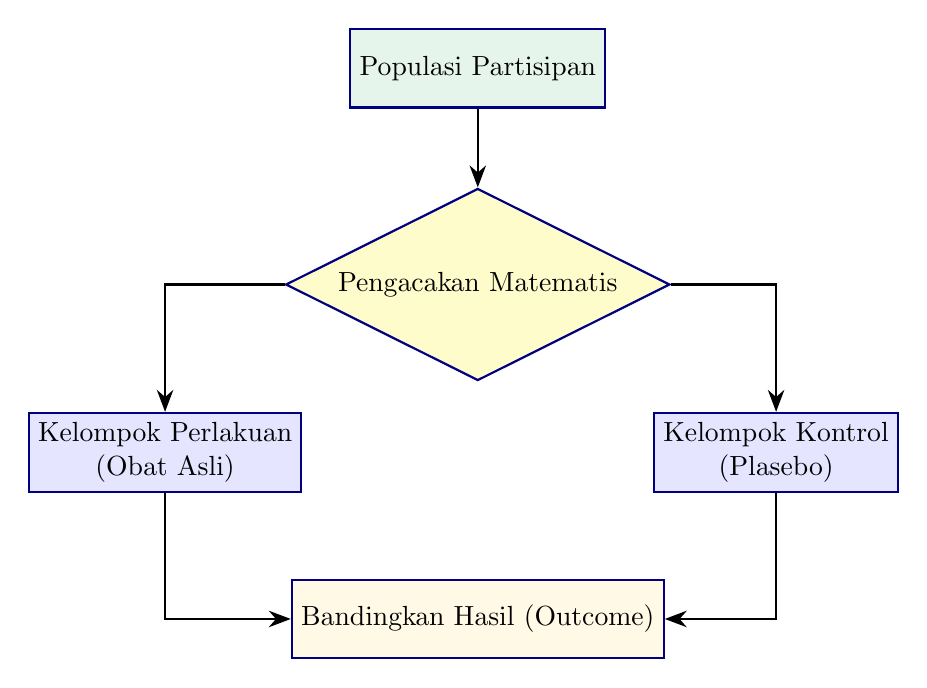
\begin{tikzpicture}[
        node distance=1cm and 1cm,
        box/.style={draw, rectangle, minimum width=2.5cm, minimum height=1cm, align=center, fill=blue!10, draw=blue!50!black, thick},
        arr/.style={-{Stealth[scale=1.2]}, thick}
    ]
    
    \node[box, fill=tipbg] (pop) {Populasi Partisipan};
    \node[box, diamond, aspect=2, fill=yellow!20] (rand) [below=1cm of pop] {Pengacakan Matematis};
    \node[box] (treat) [below left=1cm and 1cm of rand] {Kelompok Perlakuan\\(Obat Asli)};
    \node[box] (ctrl) [below right=1cm and 1cm of rand] {Kelompok Kontrol\\(Plasebo)};
    \node[box, fill=notebg] (out) [below=1cm of rand, yshift=-1.5cm] {Bandingkan Hasil (Outcome)};

    \draw[arr] (pop) -- (rand);
    \draw[arr] (rand) -| (treat);
    \draw[arr] (rand) -| (ctrl);
    \draw[arr] (treat) |- (out);
    \draw[arr] (ctrl) |- (out);

    \end{tikzpicture}
    \caption{Alur Standar \textit{Randomized Controlled Experiment} (RCT).}
\end{figure}

\textbf{Kendala Etis (Ethical Constraints):}\\
Kita tidak selalu bisa menggunakan metode ini. Sebagai contoh, sangat \textbf{tidak etis} untuk secara acak memaksa setengah dari kelompok uji untuk merokok seumur hidup mereka hanya demi membuktikan bahwa merokok menyebabkan kanker paru-paru. Dalam kasus seperti ini, peneliti harus bergantung pada data observasional yang dikontrol dengan sangat ketat.

\subsection{Contoh Modern: Uji Coba Klinis COVID-19}
Uji coba klinis untuk vaksin COVID-19 Pfizer-BioNTech adalah contoh modern yang sempurna dari eksperimen terkontrol acak tersamar ganda (\textit{randomized, double-blind controlled experiment}).
\begin{itemize}
    \item Relawan secara acak ditugaskan untuk menerima vaksin asli (perlakuan) atau suntikan plasebo yang sepenuhnya kosong (kontrol).
    \item Seiring berjalannya waktu, insiden kumulatif COVID-19 pada kelompok plasebo melonjak tajam, sementara insiden pada kelompok yang divaksinasi tetap stabil dan jauh lebih rendah. 
    \item Karena kedua kelompok ini secara praktis identik selain dari paparan vaksinnya, hal ini \textbf{membuktikan kausalitas yang ketat} bahwa vaksin tersebut mencegah penyakit.
\end{itemize}

\end{document}